%!TEX root = ../thesis.tex
%*******************************************************************************
%****************************** Third Chapter **********************************
%*******************************************************************************
\chapter{Silicon-based Sensor Technology}
\graphicspath{{3_Theory/Figs/}}

In this chapter, the High-Voltage Monolithic Active Pixel Sensors (HV-MAPS) are introduced as a particle sensing technology. The discussion begins with the fundamentals of semiconductors, followed by the principles and the electronics of HV-MAPS. The chapter then introduces the MightyPix and TelePix2 sensors - the latter being studied in details in this project.


%********************************** %First Section  **************************************
\section{Silicon Semiconductor in Particle Sensing} 
\label{section3.1}

\subsection{Silicon as a semiconductor}
A semiconductor is a material with electrical conductivity between that of a conductor and an insulator. In conductors, the Fermi level lies within a partially-filled band. In contrast, in semiconductors or insulators, it lies within the band gap between the filled valence band and the vacant conduction band. The band gap $E_G$ is given by
\begin{equation}
    E_G=E_C-E_V,
    \label{eq:bandgap}
\end{equation}
where $E_C$ is the minimum of the conduction band and $E_V$ is the maximum of the valence band. If this band gap is sufficiently small - typically less than 3 eV to 4 eV (varies in literature) - excitations can promote electrons across the gap, generating mobile charge carriers in both the valence band and the conduction band. This property defines the material as a semiconductor, and implies that its conductivity is sensitive to external factors such as temperature and external voltages. 

Silicon is a semiconductor with a band gap of 1.12 eV. It has an indirect band gap, meaning the conduction band minimum and the valence band maximum occur at different points in $\vec{k}$-space. Consequently, electron transitions across the band gap require both a photon of 1.12 eV and a phonon, or alternatively, a single photon with higher energy.


Charge carriers in semiconductors can either be intrinsic, generated by direct excitations across the band gap, or extrinsic, introduced by doping the material with other elements. Group IV semiconductors, such as silicon, can be doped with group III or V elements. 

Group III elements have one fewer valence electron than group IV elements, which creates additional electronic states above the valence band. These states are empty at 0 K, but can be occupied by electrons from the valence band at temperature $T>$0. The excitations leave behind unoccupied electronic states - equivalent to free holes - which act as positive charge carriers in the valence band. This is known as p-type doping, because the majority charge carriers (holes) carry positive charge. A small number of electrons may also be excited into the conduction band, acting as minority charge carriers.

Analogously, doping with group V elements is called n-type doping for the negatively-charged majority carriers (electrons). The additional valence electrons from dopants can occupy new states below the conduction band boundary, and can be excited to the conduction band when T$>$0. 

Both p-type and n-type doping introduce additional extrinsic charge carriers and improve the conductivity of semiconductors, particularly around room temperature. Furthermore, conductivity can be controlled by the adjusting the doping concentration, making this technique fundamental to modern semiconductor technology. 


\subsection{P-N Junction}
A p-n junction is an interface between a p-doped and a n-doped semiconductor. It functions as a diode with distinctive electrical behaviours and serves as a fundamental building block in many electronic applications. 

As discussed in the previous section, p-type and n-type semiconductors have different majority charge carriers. When the two are connected, gradients of charge carrier densities are established. The electron density is high on the n-side and low on the p-side, while the hole density shows the opposite trend. This causes electrons and holes to diffuse in opposite direction, towards each other and recombine near the junction. Each recombination removes a pair of electron and hole, and leave behind dopant ions: positive n-dopant (donor) ions and negative p-dopant (acceptor) ions. These immobile ions create an electric field that counteracts the carrier gradients and stops further diffusion. The region near the interface becomes depleted of free charge carriers - known as the depletion zone.


\begin{figure}[h!] 
\centering    
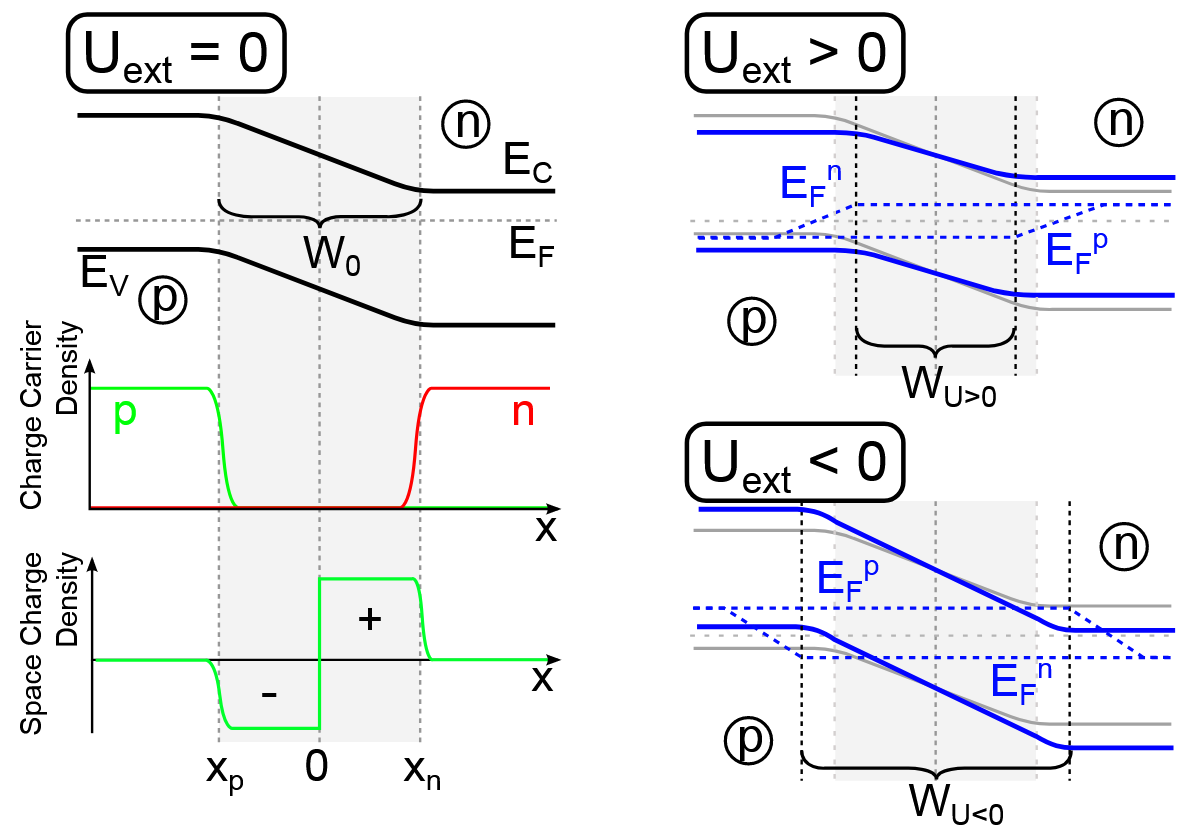
\includegraphics[width=.8\linewidth]{PNJunction}
\caption{Band diagrams of a p-n junction under different bias voltages\cite{PNJunction}. The plots of charge carrier density and space charge density of a unbiased junction are also shown on the left. $w$ is the width of the depletion zone, $x_{n,p}$ are the its widths in n,p substrates respectively. The charge carrier density is zero inside the depletion region, whereas the total charge density is zero outside. The width changes according to the sign and magnitude of bias voltage.}
\label{img:PNJunction}
\end{figure}


The effects of the carrier concentration gradient and the dopant ions in a p-n junction can be described with Poisson equation and Fick's law of diffusion. Solving these equations alongside the total charge density and boundary conditions, it's possible to determine the width of the depletion zone, $w$\footnote{For a detailed derivation, see \cite{Lutz} or \cite{Rudolf}.}:
\begin{equation}
    w = (x_p+x_n) = \sqrt{\frac{2\epsilon_0 \epsilon_r}{q} \frac{N_D + N_A}{N_D N_A} V_{contact}},
\end{equation}
where $N_{A,D}$ are the dopant densities of acceptor (p) and donor (n) respectively, $V_{contact}$ is the contact potential\footnote{Contact potential is the potential difference across a p-n junction at equilibrium and without external bias voltage. Also known as the built-in voltage.}, given by
\begin{equation}
V_{contact} = V(x_n) = \frac{2\epsilon_0 \epsilon_r}{q}(N_D x_n^2 + N_A x_p^2)
    \label{eq:contactpotential}
\end{equation}
where $\epsilon_r$ is the relative permittivity and $q$ is the electric charge of the carriers.

The width of the depletion zone can be modified by applying external bias voltages, $V_{ext}$:
\begin{equation}
    w = \sqrt{\frac{2\epsilon_0 \epsilon_r}{q} \frac{N_D + N_A}{N_D N_A} (V_{contact}-V_{ext})}
    \label{eq:DepletionWidth}
\end{equation}
if the bias voltage is small comparing to the contact potential\cite{Lutz}. The width decreases for a forward bias ($V_{ext}>0$) and increases for a reverse bias ($V_{ext}<0$).


\subsection{Application in Particle Sensing}
When a particle traverses a semiconductor, it generates charge carriers along its path, through processes such as electron-hole pair production and scattering. These charges can be efficiently separated if they are generated in the depletion region, where a non-zero electric field drives the electrons and holes in opposite directions, towards the collection electrodes.

In particle sensing applications, a wider depletion region increases the effective path length of traversing particle in the p-n junction, thereby increase the charge deposit and improve detection efficiency. This is achieved by applying reversed bias, which expands the depletion zone. However, if bias is too high, the resulting E field will be strong enough to ionise charge carriers, generating additional electron–hole pairs. This leads to an avalanche effect, causing breakdown of the sensor.



%********************************** %Second Section  *************************************
\section{HV-MAPS-based Detectors}
\label{section3.2}

HV-MAPS are fabricated using commercial CMOS technology. "High-voltage" refers to the bias voltage between the deep n-well and the substrate, typically exceeding 50 V. "Monolithic" indicates that the sensors are integrated, with the amplifier, comparator, and readout electronics built directly on the same silicon die as the sensing elements. Standard low-voltage CMOS transistors are used for the internal electronics of the chip, and floating logic is employed to bridge the high-voltage sensor with the low-voltage CMOS circuit. HV-MAPS offer several advantages, including radiation hardness, lower costs, and compact functionality, making them well-suited for particle detection and tracking applications\cite{HVMAPS}. 

The floating logic structure, illustrated in Fig. \ref{img:HVMAPS}, is used to implement the pixel architecture in HV-MAPS. The pixel's sensing element is a p-n junction formed by a deep n-well within a p-doped substrate. It is reverse-biased with a high voltage close to the breakdown voltage, to extend the depletion region deep into the lowly doped substrate. For example, under a 60 V bias, the depletion zone can reach a thickness of approximately 9$\mu$m. A particle  traversing this region can generate relatively large signal, on the order of 700 e\cite{HVMAPS2}. The high electric field in the depletion zone allows charge carriers to be collected by drift, with the n-well serving as the cathode. This drift-based collection enables faster signal response comparing to low-voltage triple-well MAPS, where charge collection relies on slower diffusion mechanisms.


\begin{figure}[h!]
\centering
\begin{subfigure}{.49\textwidth}
  \centering
  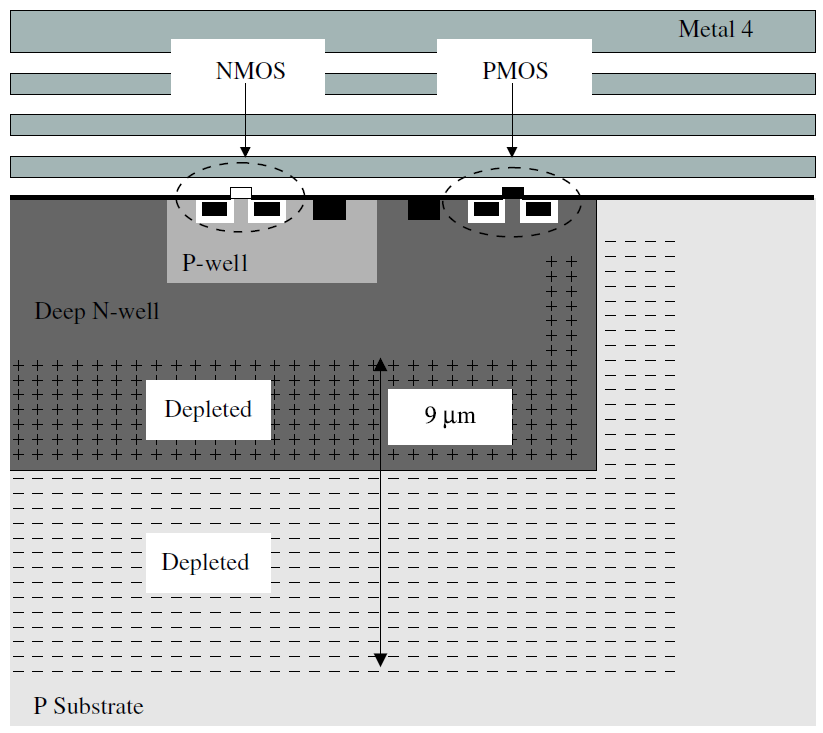
\includegraphics[width=1.0\linewidth]{FloatingLogic}
  \caption{The floating logic, including the sensing diode. The plus and minus signs denote the area with non-zero total charge density - the depletion region.}
\end{subfigure}
\begin{subfigure}{.49\textwidth}
  \centering
  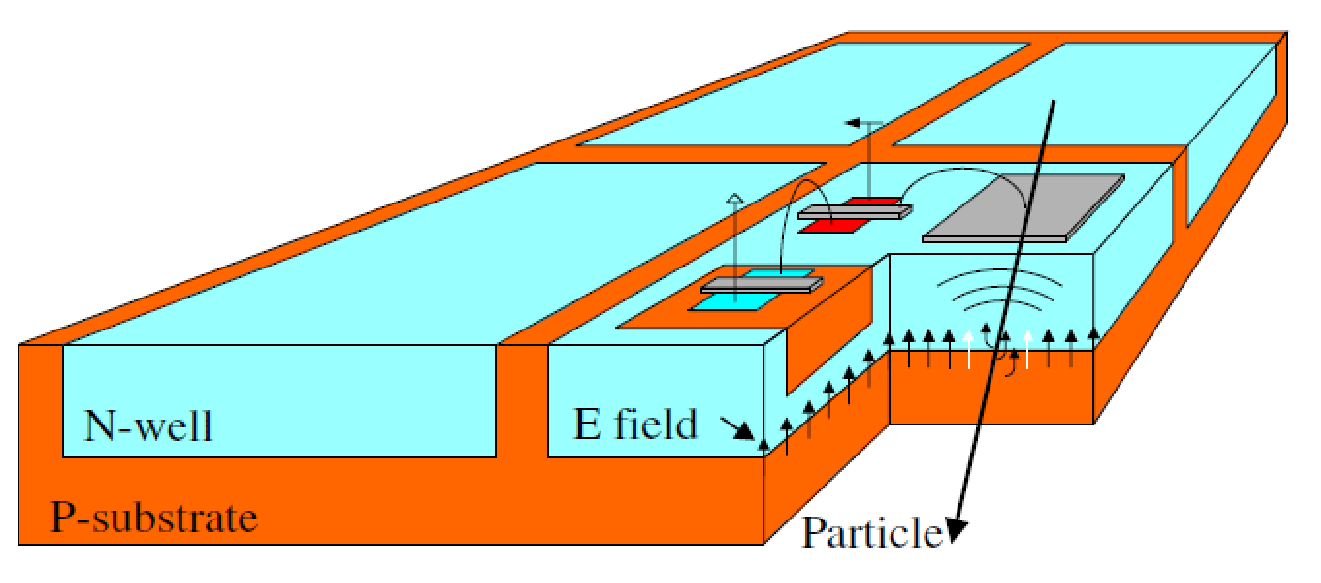
\includegraphics[width=1.0\linewidth]{HVMAPS}
  \caption{Four high-voltage pixels.}
\end{subfigure}
\caption{The pixel structure of HV-MAPS\cite{HVMAPS2}.}
\label{img:HVMAPS}
\end{figure}


An arbitrarily complex CMOS readout circuits can be implemented within the deep n-well, allowing fully integrated signal processing. A simplified block diagram of the pixel architecture is shown in Fig. \ref{img:Readout}. The separated charges are first collected by the p-type and n-type MOSFET (PMOS and NMOS) embedded within the N-well, producing a short current pulse. During this stage, charge sharing between neighbouring pixels may occur. The signal is then processed by a charge-sensitive amplifier (CSA), which integrates the incoming charge and converts it into a proportional voltage signal. Next, the voltage is sent to a comparator, which compares the signal with the threshold (THL) value and digitises it. Finally, the signal is passed to the readout, in which pixel address, time-of-arrival (ToA), and collected charge are assigned.

\begin{figure}
\centering    
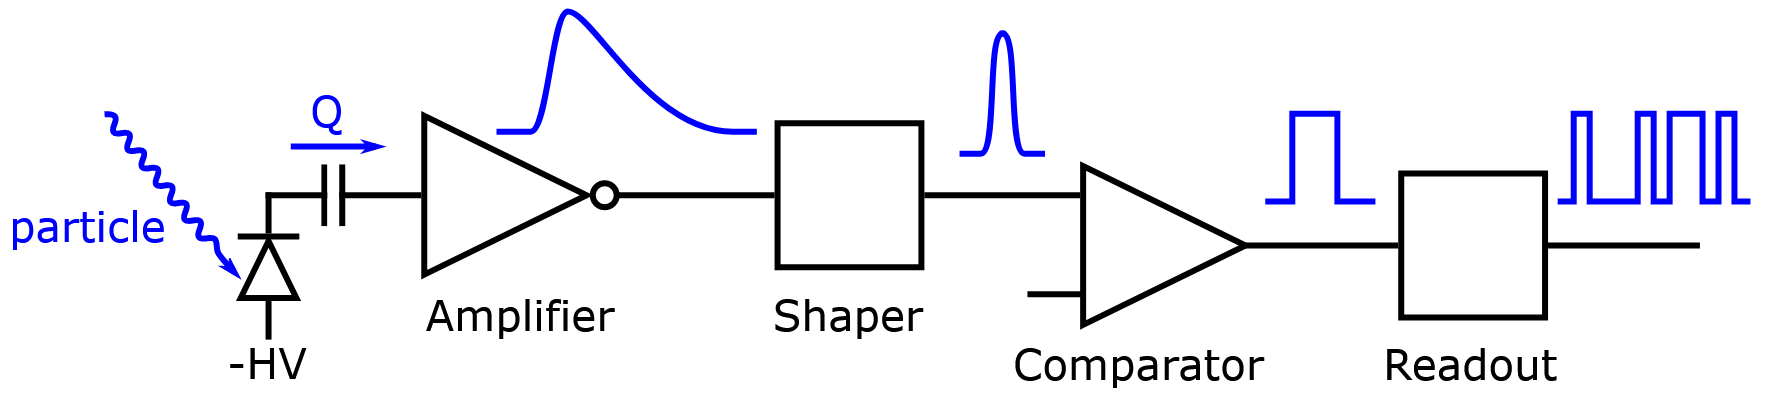
\includegraphics[width=1\linewidth]{Readout}
\caption{A simplified block diagram of the pixel\cite{Rudolf}. The signal processing and readout circuitry are integrated in the same silicon die as the sensor diode.}
\label{img:Readout}
\end{figure}


The charge of a signal is represented by threshold-over-time (ToT), which is linearly proportional to its energy and can be calibrated at a test beam. The readout is triggered when the output voltage exceeds the predefined threshold. The rise time of a signal - the time taken to reach the peak output voltage - depends on factors such as the capacitance and transconductance of the amplifier, but is independent of the input charge (see \cite{RiseTime}). The amount of charge affects only the peak output voltage. As a result, high-charge signals remain above the threshold for longer duration than those with lower charge, as shown in Fig. \ref{img:Timewalk}. Therefore, ToT is a reliable proxy for the deposited charge. 

However, for the same reason, the time at which a signal crosses the threshold also depends on its amplitude. Since this crossing time is used to determine signal's time-of-arrival (ToA), the measured timing becomes dependent on ToT. Low-charge signals exhibit larger time delays comparing to high-charge signals. This phenomenon is known as the time-walk effect, and must be corrected for to achieve accurate timing.


\begin{figure}[h!]
\centering
\begin{subfigure}{.55\textwidth}
  \centering
  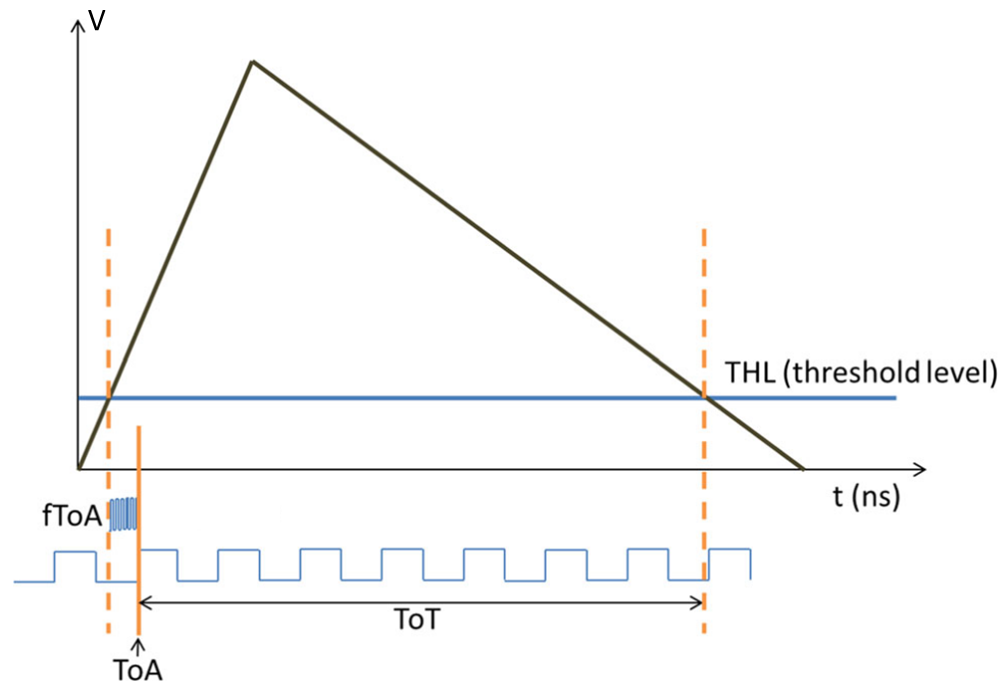
\includegraphics[width=1.0\linewidth]{Signal}
  \caption{Timing measurement of a single signal, showing the threshold crossing used to determine the Time-of-Arrival (ToA).}
\end{subfigure}
\begin{subfigure}{.44\textwidth}
  \centering
  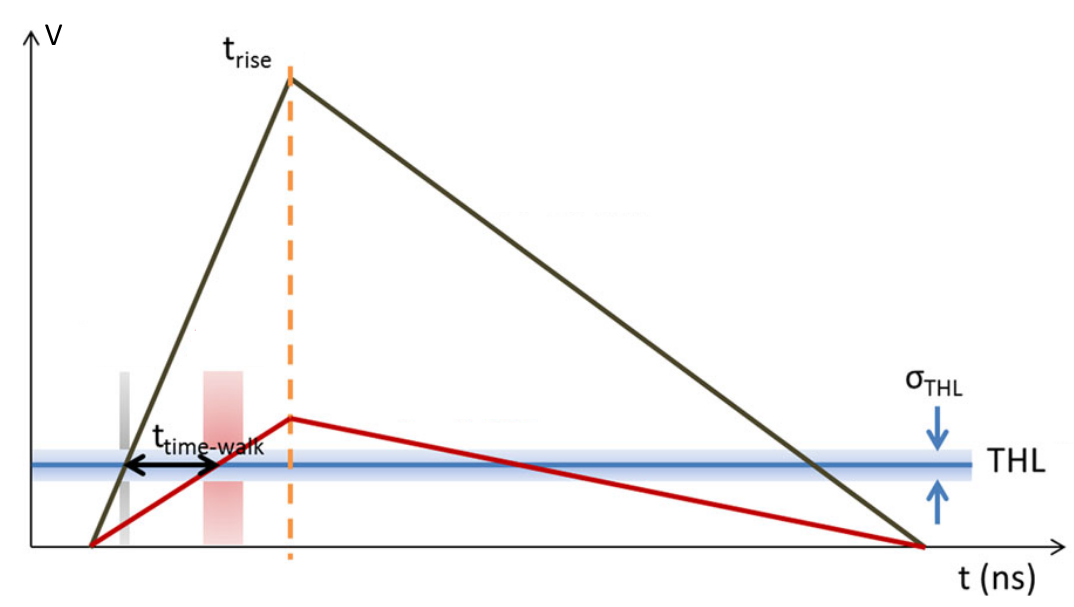
\includegraphics[width=1.0\linewidth]{Timewalk}
  \caption{An illustration of the time-walk effect. The brown line represents a high-charge signal, while the red line represents a low-charge signal. The difference in threshold-crossing times demonstrates the charge-dependent delay in signal detection.}
\end{subfigure}
\caption{Illustrations of timing characteristics in HV-MAPS readout\cite{Timewalk}.}
\label{img:Timewalk}
\end{figure}


%%% Not sure if this is important...
%The integrity of sensing and readout components significantly reduces the material budget from silicon wafers and precision bonding – HV-CMOS MAPS may be thinned down to 50$\mu$m\cite{Mupix2}; this is when the handling of the sensor because a limiting factor, rather than the sensor itself. However, the periphery of the sensor, where the readout circuitry, wire bonding, etc. are packed, will be insensitive to the signal. This requires some attention when designing the layout of the chip.

%%% If needed, talk about the noise as well? The jitter - they lead to the distribution in the time resolution anyway...


%********************************** % Third Section  *************************************
\section{MightyPix and TelePix2}  
\label{section3.3}

%% Talk about the similarities and difference between Telepix2 and MightyPix, refer to different lits.

Building on the developments of MuPix\cite{Mupix}\cite{Mupix2} and ATLASPix\cite{ATLASPix}\cite{MupixATLASPix}, MightyPix is a family of HV-CMOS MAPS sensors designed to meet the requirements of radiation hardness, timing, and granularity in the central pixelated region of the Mighty Tracker Stations. MightyPix1 is the first HV-MAPS sensor designed for LHCb\cite{MightypixUpdate}, developed by the ASIC and Detector Laboratory at the Karlsruhe Institute of Technology (KIT)\cite{KIT}. 

The performance of MightyPix is interested; however, only 16 working chips are available, which is insufficient to carry out a radiation damage study. Instead, TelePix, a related family of HV-CMOS MAPS with a similar design\footnote{For a comparison between MightyPix and TelePix2, please refer to \cite{Mightypix}\cite{TP2manual}.}, is more widely available. In this project, the time resolution of TelePix2 was evaluated to gain insight into the timing performance of sensors of this type.

The TelePix family is designed to serve as telescope planes in the DESY II Test Beam Facility to solve the problem from separated telescope and trigger plane\cite{Telepix}. It is designed by KIT and further developed in collaboration with Heidelberg University and DESY\cite{DESYreport}. The latest version, TelePix2, offers several key features, including high-resolution time sampling, fast signal output, a user-configurable trigger (e.g., pixel masking), and low material budget. The parameters are summarised in Table \ref{Table:TP2}.



\begin{table}[h!]
\centering
\begin{tabular}{||c | c | c | c||} 
\hline
 Technology & Pixel dimension & Chip dimension & Pixels per chip \\
 \hline
180nm HV-CMOS & $165 \times 25 \: \mu m^{2}$ & $20 \times 13 \: mm^{2}$ & $ 120 \times 400$\\ [1ex]
\hline
\end{tabular}

\vspace{0.6em}

\begin{tabular}{||c | c | c||}
\hline
TDC bandwidth & Maximum HV bias & Material budget\\
\hline
125Hz(4ns) & -90V/-150V (pixel/chip) &  0.0011 from $100 \: \mu m$ silicon \\[1ex]
\hline
\end{tabular}
\caption{The parameters of TelePix2\cite{Telepix}\cite{teststart}.}
\label{Table:TP2}
\end{table}
